\documentclass{standalone}
\usepackage{tikz}
\usetikzlibrary{patterns, positioning}


\begin{document}
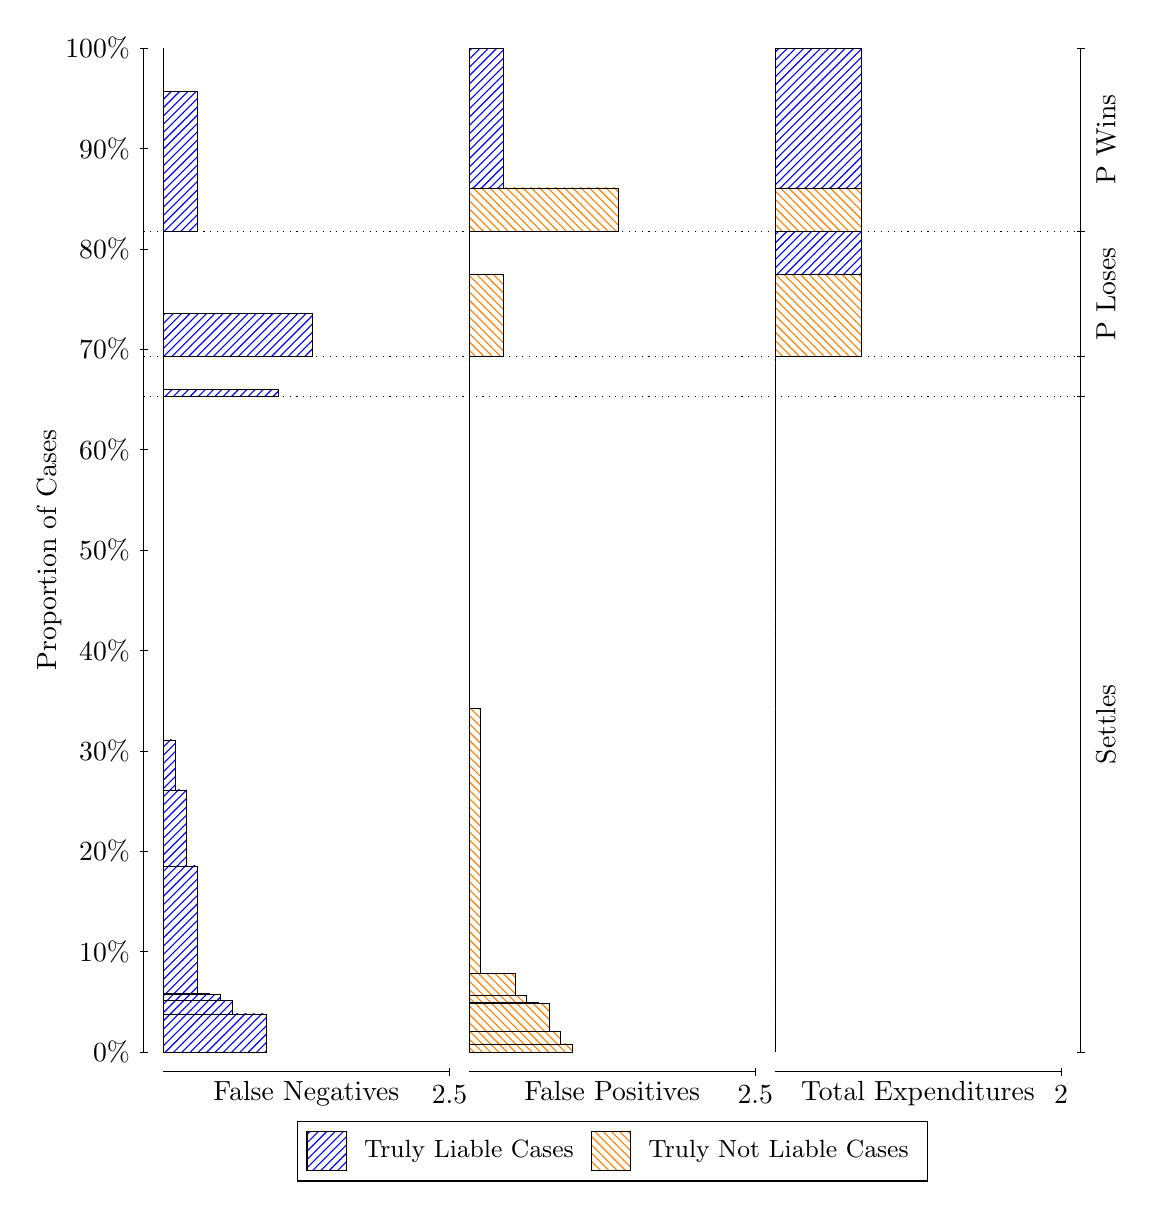
\begin{tikzpicture}
\draw[black, very thin] (1.5,1.75) -- (1.5,14.5);
\node[rotate=90, text=black, anchor=center] at (0.3, 8.125) {Proportion of Cases};
\draw[black, very thin] (1.45,1.75) -- (1.55,1.75);
\node[text=black, anchor=east] at (1.45, 1.75) {0\%};
\draw[black, very thin] (1.45,3.025) -- (1.55,3.025);
\node[text=black, anchor=east] at (1.45, 3.025) {10\%};
\draw[black, very thin] (1.45,4.3) -- (1.55,4.3);
\node[text=black, anchor=east] at (1.45, 4.3) {20\%};
\draw[black, very thin] (1.45,5.575) -- (1.55,5.575);
\node[text=black, anchor=east] at (1.45, 5.575) {30\%};
\draw[black, very thin] (1.45,6.85) -- (1.55,6.85);
\node[text=black, anchor=east] at (1.45, 6.85) {40\%};
\draw[black, very thin] (1.45,8.125) -- (1.55,8.125);
\node[text=black, anchor=east] at (1.45, 8.125) {50\%};
\draw[black, very thin] (1.45,9.4) -- (1.55,9.4);
\node[text=black, anchor=east] at (1.45, 9.4) {60\%};
\draw[black, very thin] (1.45,10.675) -- (1.55,10.675);
\node[text=black, anchor=east] at (1.45, 10.675) {70\%};
\draw[black, very thin] (1.45,11.95) -- (1.55,11.95);
\node[text=black, anchor=east] at (1.45, 11.95) {80\%};
\draw[black, very thin] (1.45,13.225) -- (1.55,13.225);
\node[text=black, anchor=east] at (1.45, 13.225) {90\%};
\draw[black, very thin] (1.45,14.5) -- (1.55,14.5);
\node[text=black, anchor=east] at (1.45, 14.5) {100\%};

\draw[black, very thin] (13.4,1.75) -- (13.4,14.5);
\draw[black, very thin] (13.35,1.75) -- (13.45,1.75);
\node[anchor=west] at (13.35, 1.75) {};
\draw[black, very thin] (13.35,10.075) -- (13.45,10.075);
\node[anchor=west] at (13.35, 10.075) {};
\draw[black, very thin] (13.35,10.585) -- (13.45,10.585);
\node[anchor=west] at (13.35, 10.585) {};
\draw[black, very thin] (13.35,12.174) -- (13.45,12.174);
\node[anchor=west] at (13.35, 12.174) {};
\draw[black, very thin] (13.35,14.5) -- (13.45,14.5);
\node[anchor=west] at (13.35, 14.5) {};

\draw[black, very thin, pattern color=blue, pattern=north east lines] (1.75,1.75) rectangle (3.058,2.2347);
\draw[black, very thin, pattern color=blue, pattern=north east lines] (1.75,2.2347) rectangle (2.622,2.4038);
\draw[black, very thin, pattern color=blue, pattern=north east lines] (1.75,2.4038) rectangle (2.4767,2.4855);
\draw[black, very thin, pattern color=blue, pattern=north east lines] (1.75,2.4855) rectangle (2.3313,2.4926);
\draw[black, very thin, pattern color=blue, pattern=north east lines] (1.75,2.4926) rectangle (2.186,4.113);
\draw[black, very thin, pattern color=blue, pattern=north east lines] (1.75,4.113) rectangle (2.0407,5.0773);
\draw[black, very thin, pattern color=blue, pattern=north east lines] (1.75,5.0773) rectangle (1.8953,5.7136);
\draw[black, very thin, pattern color=orange, pattern=north west lines] (1.75,5.7136) rectangle (1.75,10.075);
\draw[black, very thin, pattern color=blue, pattern=north east lines] (1.75,10.075) rectangle (3.2033,10.165);
\draw[black, very thin, pattern color=orange, pattern=north west lines] (1.75,10.165) rectangle (1.75,10.585);
\draw[black, very thin, pattern color=blue, pattern=north east lines] (1.75,10.585) rectangle (3.6393,11.129);
\draw[black, very thin, pattern color=orange, pattern=north west lines] (1.75,11.129) rectangle (1.75,12.174);
\draw[black, very thin, pattern color=blue, pattern=north east lines] (1.75,12.174) rectangle (2.186,13.952);
\draw[black, very thin, pattern color=orange, pattern=north west lines] (1.75,13.952) rectangle (1.75,14.5);
\draw[black, very thin, pattern color=orange, pattern=north west lines] (5.6333,1.75) rectangle (6.9413,1.853);
\draw[black, very thin, pattern color=orange, pattern=north west lines] (5.6333,1.853) rectangle (6.796,2.0156);
\draw[black, very thin, pattern color=orange, pattern=north west lines] (5.6333,2.0156) rectangle (6.6507,2.3705);
\draw[black, very thin, pattern color=orange, pattern=north west lines] (5.6333,2.3705) rectangle (6.5053,2.3784);
\draw[black, very thin, pattern color=orange, pattern=north west lines] (5.6333,2.3784) rectangle (6.36,2.4643);
\draw[black, very thin, pattern color=orange, pattern=north west lines] (5.6333,2.4643) rectangle (6.2147,2.744);
\draw[black, very thin, pattern color=orange, pattern=north west lines] (5.6333,2.744) rectangle (5.7787,6.1114);
\draw[black, very thin, pattern color=blue, pattern=north east lines] (5.6333,6.1114) rectangle (5.6333,10.075);
\draw[black, very thin, pattern color=orange, pattern=north west lines] (5.6333,10.075) rectangle (5.6333,10.495);
\draw[black, very thin, pattern color=blue, pattern=north east lines] (5.6333,10.495) rectangle (5.6333,10.585);
\draw[black, very thin, pattern color=orange, pattern=north west lines] (5.6333,10.585) rectangle (6.0693,11.63);
\draw[black, very thin, pattern color=blue, pattern=north east lines] (5.6333,11.63) rectangle (5.6333,12.174);
\draw[black, very thin, pattern color=orange, pattern=north west lines] (5.6333,12.174) rectangle (7.5227,12.723);
\draw[black, very thin, pattern color=blue, pattern=north east lines] (5.6333,12.723) rectangle (6.0693,14.5);
\draw[black, very thin, pattern color=orange, pattern=north west lines] (9.5167,1.75) rectangle (9.5167,6.1114);
\draw[black, very thin, pattern color=blue, pattern=north east lines] (9.5167,6.1114) rectangle (9.5167,10.075);
\draw[black, very thin, pattern color=orange, pattern=north west lines] (9.5167,10.075) rectangle (9.5167,10.495);
\draw[black, very thin, pattern color=blue, pattern=north east lines] (9.5167,10.495) rectangle (9.5167,10.585);
\draw[black, very thin, pattern color=orange, pattern=north west lines] (9.5167,10.585) rectangle (10.607,11.63);
\draw[black, very thin, pattern color=blue, pattern=north east lines] (9.5167,11.63) rectangle (10.607,12.174);
\draw[black, very thin, pattern color=orange, pattern=north west lines] (9.5167,12.174) rectangle (10.607,12.723);
\draw[black, very thin, pattern color=blue, pattern=north east lines] (9.5167,12.723) rectangle (10.607,14.5);
\draw[black, dotted] (1.5,10.075) -- (13.4,10.075);
\draw[black, dotted] (1.5,10.585) -- (13.4,10.585);
\draw[black, dotted] (1.5,12.174) -- (13.4,12.174);
\draw[black, very thin] (1.75,1.5) -- (5.3833,1.5);
\node[text=black, anchor=north] at (3.5667, 1.5) {False Negatives};
\draw[black, very thin] (5.3833,1.45) -- (5.3833,1.55);
\node[text=black, anchor=north] at (5.3833, 1.45) {2.5};

\draw[black, very thin] (5.6333,1.5) -- (9.2667,1.5);
\node[text=black, anchor=north] at (7.45, 1.5) {False Positives};
\draw[black, very thin] (9.2667,1.45) -- (9.2667,1.55);
\node[text=black, anchor=north] at (9.2667, 1.45) {2.5};

\draw[black, very thin] (9.5167,1.5) -- (13.15,1.5);
\node[text=black, anchor=north] at (11.333, 1.5) {Total Expenditures};
\draw[black, very thin] (13.15,1.45) -- (13.15,1.55);
\node[text=black, anchor=north] at (13.15, 1.45) {2};

\node[text=black, centered, rotate=90] at (13.72, 5.9125) {Settles};

\node[text=black, centered, rotate=90] at (13.72, 11.379) {P Loses};
\node[text=black, centered, rotate=90] at (13.72, 13.337) {P Wins};

\draw (7.449999999999999,1.5) node[draw=none] (baseCoordinate) {};
\begin{scope}[align=center]
        \matrix[scale=0.5, draw=black, below=0.5cm of baseCoordinate, nodes={draw}, column sep=0.1cm]{
            \node[rectangle, draw, minimum width=0.5cm, minimum height=0.5cm, pattern color=blue, pattern=north east lines] {}; &
            \node[draw=none, font=\small, text=black] (B) {Truly Liable Cases}; &
            \node[rectangle, draw, minimum width=0.5cm, minimum height=0.5cm, pattern color=orange, pattern=north west lines] {}; &
            \node[draw=none, font=\small, text=black] (B) {Truly Not Liable Cases}; \\
            };
\end{scope}

\end{tikzpicture}
\end{document}